%==============================================================================
% Tento soubor použijte jako základ
% This file should be used as a base for the thesis
% Autoři / Authors: 2008 Michal Bidlo, 2022 Jaroslav Dytrych
% Kontakt pro dotazy a připomínky: sablona@fit.vutbr.cz
% Contact for questions and comments: sablona@fit.vutbr.cz
%==============================================================================
% kódování: UTF-8 (zmena prikazem iconv, recode nebo cstocs)
% encoding: UTF-8 (you can change it by command iconv, recode or cstocs)
%------------------------------------------------------------------------------
% zpracování / processing: make, make pdf, make clean
%==============================================================================
% Soubory, které je nutné upravit nebo smazat: / Files which have to be edited or deleted:
%   projekt-20-literatura-bibliography.bib - literatura / bibliography
%   projekt-01-kapitoly-chapters.tex - obsah práce / the thesis content
%   projekt-01-kapitoly-chapters-en.tex - obsah práce v angličtině / the thesis content in English
%   projekt-30-prilohy-appendices.tex - přílohy / appendices
%   projekt-30-prilohy-appendices-en.tex - přílohy v angličtině / appendices in English
%==============================================================================
%\documentclass[]{fitthesis} % bez zadání - pro začátek práce, aby nebyl problém s překladem
%\documentclass[english]{fitthesis} % without assignment - for the work start to avoid compilation problem
\documentclass[zadani]{fitthesis} % odevzdani do IS VUT a/nebo tisk s barevnými odkazy - odkazy jsou barevné
%\documentclass[english,zadani]{fitthesis} % for submission to the IS VUT and/or print with color links - links are color
%\documentclass[zadani,print]{fitthesis} % pro černobílý tisk - odkazy jsou černé
%\documentclass[english,zadani,print]{fitthesis} % for the black and white print - links are black
%\documentclass[zadani,cprint]{fitthesis} % pro barevný tisk - odkazy jsou černé, znak VUT barevný
%\documentclass[english,zadani,cprint]{fitthesis} % for the print - links are black, logo is color
% * Je-li práce psaná v anglickém jazyce, je zapotřebí u třídy použít 
%   parametr english následovně:
%   If thesis is written in English, it is necessary to use 
%   parameter english as follows:
%      \documentclass[english]{fitthesis}
% * Je-li práce psaná ve slovenském jazyce, je zapotřebí u třídy použít 
%   parametr slovak následovně:
%   If the work is written in the Slovak language, it is necessary 
%   to use parameter slovak as follows:
%      \documentclass[slovak]{fitthesis}
% * Je-li práce psaná v anglickém jazyce se slovenským abstraktem apod., 
%   je zapotřebí u třídy použít parametry english a enslovak následovně:
%   If the work is written in English with the Slovak abstract, etc., 
%   it is necessary to use parameters english and enslovak as follows:
%      \documentclass[english,enslovak]{fitthesis}

% Základní balíčky jsou dole v souboru šablony fitthesis.cls
% Basic packages are at the bottom of template file fitthesis.cls
% zde můžeme vložit vlastní balíčky / you can place own packages here


% Pro seznam zkratek lze využít balíček Glossaries - nutno odkomentovat i níže a při kompilaci z konzoly i v Makefile (plnou verzi pro Perl, nebo lite)
% The Glossaries package can be used for the list of abbreviations - it is necessary to uncomment also below. When compiling from the console also in the Makefile (full version for Perl or lite)
%\usepackage{glossaries}
%\usepackage{glossary-superragged}
%\makeglossaries 

% Nastavení cesty k obrázkům
% Setting of a path to the pictures
%\graphicspath{{obrazky-figures/}{./obrazky-figures/}}
%\graphicspath{{obrazky-figures/}{../obrazky-figures/}}

%---rm---------------
\renewcommand{\rmdefault}{lmr}%zavede Latin Modern Roman jako rm / set Latin Modern Roman as rm
%---sf---------------
\renewcommand{\sfdefault}{qhv}%zavede TeX Gyre Heros jako sf
%---tt------------
\renewcommand{\ttdefault}{lmtt}% zavede Latin Modern tt jako tt

% vypne funkci šablony, která automaticky nahrazuje uvozovky,
% aby nebyly prováděny nevhodné náhrady v popisech API apod.
% disables function of the template which replaces quotation marks
% to avoid unnecessary replacements in the API descriptions etc.
\csdoublequotesoff

\usepackage{url}
\usepackage[inkscapelatex=false]{svg}
\usepackage{comment}
\usepackage{listings}
\usepackage{subcaption}
\usepackage{lipsum}

% =======================================================================
% balíček "hyperref" vytváří klikací odkazy v pdf, pokud tedy použijeme pdflatex
% problém je, že balíček hyperref musí být uveden jako poslední, takže nemůže
% být v šabloně
% "hyperref" package create clickable links in pdf if you are using pdflatex.
% Problem is that this package have to be introduced as the last one so it 
% can not be placed in the template file.
\ifWis
\ifx\pdfoutput\undefined % nejedeme pod pdflatexem / we are not using pdflatex
\else
  \usepackage{color}
  \usepackage[unicode,colorlinks,hyperindex,plainpages=false,pdftex]{hyperref}
  \definecolor{hrcolor-ref}{RGB}{223,52,30}
  \definecolor{hrcolor-cite}{HTML}{2F8F00}
  \definecolor{hrcolor-urls}{HTML}{092EAB}
  \hypersetup{
	linkcolor=hrcolor-ref,
	citecolor=hrcolor-cite,
	filecolor=magenta,
	urlcolor=hrcolor-urls
  }
  \def\pdfBorderAttrs{/Border [0 0 0] }  % bez okrajů kolem odkazů / without margins around links
  \pdfcompresslevel=9
\fi
\else % pro tisk budou odkazy, na které se dá klikat, černé / for the print clickable links will be black
\ifx\pdfoutput\undefined % nejedeme pod pdflatexem / we are not using pdflatex
\else
  \usepackage{color}
  \usepackage[unicode,colorlinks,hyperindex,plainpages=false,pdftex,urlcolor=black,linkcolor=black,citecolor=black]{hyperref}
  \definecolor{links}{rgb}{0,0,0}
  \definecolor{anchors}{rgb}{0,0,0}
  \def\AnchorColor{anchors}
  \def\LinkColor{links}
  \def\pdfBorderAttrs{/Border [0 0 0] } % bez okrajů kolem odkazů / without margins around links
  \pdfcompresslevel=9
\fi
\fi
% Řešení problému, kdy klikací odkazy na obrázky vedou za obrázek
% This solves the problems with links which leads after the picture
\usepackage[all]{hypcap}


% Informace o práci/projektu / Information about the thesis
%---------------------------------------------------------------------------
\projectinfo{
  %Prace / Thesis
  project={SP},            %typ práce BP/SP/DP/DR  / thesis type (SP = term project)
  year={2023},             % rok odevzdání / year of submission
  date=\today,             % datum odevzdání / submission date
  %Nazev prace / thesis title
  title.cs={Vizualizační nástroj pro pilota dronu \\v Microsoft HoloLens 2},  % název práce v češtině či slovenštině (dle zadání) / thesis title in czech language (according to assignment)
  title.en={Visualization Tool for a Drone Pilot in Microsoft HoloLens 2}, % název práce v angličtině / thesis title in english
  %title.length={14.5cm}, % nastavení délky bloku s titulkem pro úpravu zalomení řádku (lze definovat zde nebo níže) / setting the length of a block with a thesis title for adjusting a line break (can be defined here or below)
  %sectitle.length={14.5cm}, % nastavení délky bloku s druhým titulkem pro úpravu zalomení řádku (lze definovat zde nebo níže) / setting the length of a block with a second thesis title for adjusting a line break (can be defined here or below)
  %dectitle.length={14.5cm}, % nastavení délky bloku s titulkem nad prohlášením pro úpravu zalomení řádku (lze definovat zde nebo níže) / setting the length of a block with a thesis title above declaration for adjusting a line break (can be defined here or below)
  %Autor / Author
  author.name={Jakub},   % jméno autora / author name
  author.surname={Komárek},   % příjmení autora / author surname 
  author.title.p={Bc.}, % titul před jménem (nepovinné) / title before the name (optional)
  %author.title.a={Ph.D.}, % titul za jménem (nepovinné) / title after the name (optional)
  %Ustav / Department
  department={UPGM}, % doplňte příslušnou zkratku dle ústavu na zadání: UPSY/UIFS/UITS/UPGM / fill in appropriate abbreviation of the department according to assignment: UPSY/UIFS/UITS/UPGM
  % Školitel / supervisor
  supervisor.name={Daniel},   % jméno školitele / supervisor name 
  supervisor.surname={Bambušek},   % příjmení školitele / supervisor surname
  supervisor.title.p={Ing.},   %titul před jménem (nepovinné) / title before the name (optional)
  %supervisor.title.a={},    %titul za jménem (nepovinné) / title after the name (optional)
  % Klíčová slova / keywords
  keywords.cs={Microsoft HoloLens 2, Unity, C\#, Dron, Rozšířená realita, DJI drony, Vizualizace letových veličin, návrh UI }, % klíčová slova v českém či slovenském jazyce / keywords in czech or slovak language
  keywords.en={Microsoft HoloLens 2, Unity, C\#, Drone, DJI drones, Visualisation of flight variables, UI design, Augmented Reality }, % klíčová slova v anglickém jazyce / keywords in english
  %keywords.en={Here, individual keywords separated by commas will be written in English.},
  % Abstrakt / Abstract
abstract.cs={Cílem práce je tvorba moderního nástroje pro usnadnění obsluhy dronu zejména v profesní sféře. Nástroj, který autor tvořil, si klade za cíl usnadnit plánovací rutinu obvyklých misí a pomoci při jejím bezpečném plněním. Nástroj byl vytvořen i s ohledem na legislativní omezení provozu dronů a přispívá k jejich korektnímu dodržování. 
Problematiku autor řešil za pomocí vytvořené klient-server aplikace v prostředí virtuální rozšířené reality v brýlích Hololens 2. Pomoc při pilotáži má přinést dynamický HUD, který se pohybuje spolu s dronem a okolo něho zobrazuje letové  veličiny spolu s video přenosem z kamery drona. 
Ke snadnějšímu plánování misí má přispět implementovaná 3D minimapa, která informace o plánované misi promítá do světa v okolí pilota.
Práce je experimentálního charakteru a má za úkol zjistit použitelnost rozšířené reality při profesní obsluze drona. Výsledky budou zjištěny za pomocí rozsáhlého uživatelského testování, v rámci kterého dojde k porovnání stávající aplikace Lichi s vyvíjenou aplikaci v rámci připravených testovacích scénářů.  }, % abstrakt v českém či slovenském jazyce / abstract in czech or slovak language
abstract.en={The aim of the work is to create a modern tool to facilitate the operation of drones, especially in the professional sphere. The tool created by the author aims to facilitate the planning routine of the usual missions and to help in its safe execution. The tool has also been created taking into account the legislative restrictions on drone operation and contributes to their correct compliance. 
The author solved the problem using a developed client-server application in a virtual augmented reality environment in Hololens 2 glasses. The assistance in piloting is to be provided by a dynamic HUD that moves with the drone and displays flight variables around it together with the video transmission from the drone's camera. 
To facilitate mission planning, a 3D minimap is implemented that projects information about the planned mission into the world around the pilot.
The work is experimental in nature and is intended to determine the applicability of augmented reality in the professional operation of the drone. The results will be determined through extensive user testing, which will compare the existing Lichi application with the application under development in prepared test scenarios.}, % abstrakt v anglickém jazyce / abstract in english  %abstract.en={An abstract of the work in English will be written in this paragraph.},
  % Prohlášení (u anglicky psané práce anglicky, u slovensky psané práce slovensky; u projektové praxe lze zakomentovat) / Declaration (for thesis in english should be in english; for project practice can be commented out)
  declaration={Prohlašuji, že jsem tuto bakalářskou práci vypracoval samostatně pod vedením pana Ing. Daniela Bambuška.
Uvedl jsem všechny literární prameny, publikace a další zdroje, ze kterých jsem čerpal.},
  %declaration={I hereby declare that this Bachelor's thesis was prepared as an original work by the author under the supervision of Mr. X
% The supplementary information was provided by Mr. Y
% I have listed all the literary sources, publications and other sources, which were used during the preparation of this thesis.},
  % Poděkování (nepovinné, nejlépe v jazyce práce; nechcete-li, zakomentujte pro skrytí nadpisu) / Acknowledgement (optional, ideally in the language of the thesis; comment out for hiding including heading)
  acknowledgment={Děkuji panu Ing. Danielu Bambuškovi za odborné konzultace a pomoc při tvorbě práce.
 },
  %acknowledgment={Here it is possible to express thanks to the supervisor and to the people which provided professional help
%(external submitter, consultant, etc.).},
  % Rozšířený abstrakt (cca 3 normostrany) - lze definovat zde nebo níže / Extended abstract (approximately 3 standard pages) - can be defined here or below
  %extendedabstract={Do tohoto odstavce bude zapsán rozšířený výtah (abstrakt) práce v českém (slovenském) jazyce.},
  %extabstract.odd={true}, % Začít rozšířený abstrakt na liché stránce? / Should extended abstract start on the odd page?
  %faculty={FIT}, % FIT/FEKT/FSI/FA/FCH/FP/FAST/FAVU/USI/DEF
  faculty.cs={Fakulta informačních technologií}, % Fakulta v češtině - pro využití této položky výše zvolte fakultu DEF / Faculty in Czech - for use of this entry select DEF above
  faculty.en={Faculty of Information Technology}, % Fakulta v angličtině - pro využití této položky výše zvolte fakultu DEF / Faculty in English - for use of this entry select DEF above
  department.cs={Ústav počítačové grafiky a multimédií}, % Ústav v češtině - pro využití této položky výše zvolte ústav DEF nebo jej zakomentujte / Department in Czech - for use of this entry select DEF above or comment it out
  department.en={Department of Computer Graphics and Multimedia} % Ústav v angličtině - pro využití této položky výše zvolte ústav DEF nebo jej zakomentujte / Department in English - for use of this entry select DEF above or comment it out
}

% Rozšířený abstrakt (cca 3 normostrany) - lze definovat zde nebo výše / Extended abstract (approximately 3 standard pages) - can be defined here or above
%\extendedabstract{Do tohoto odstavce bude zapsán výtah (abstrakt) práce v českém (slovenském) jazyce.}
% Začít rozšířený abstrakt na liché stránce? / Should extended abstract start on the odd page?
%\extabstractodd{true}

% nastavení délky bloku s titulkem pro úpravu zalomení řádku - lze definovat zde nebo výše / setting the length of a block with a thesis title for adjusting a line break - can be defined here or above
%\titlelength{14.5cm}
% nastavení délky bloku s druhým titulkem pro úpravu zalomení řádku - lze definovat zde nebo výše / setting the length of a block with a second thesis title for adjusting a line break - can be defined here or above
%\sectitlelength{14.5cm}
% nastavení délky bloku s titulkem nad prohlášením pro úpravu zalomení řádku - lze definovat zde nebo výše / setting the length of a block with a thesis title above declaration for adjusting a line break - can be defined here or above
%\dectitlelength{14.5cm}

% řeší první/poslední řádek odstavce na předchozí/následující stránce
% solves first/last row of the paragraph on the previous/next page
\clubpenalty=10000
\widowpenalty=10000

% checklist
\newlist{checklist}{itemize}{1}
\setlist[checklist]{label=$\square$}

% Kompilace po částech (rychlejší, ale v náhledu nemusí být vše aktuální)
% Compilation piecewise (faster, but not all parts in preview will be up-to-date)
% Další informace viz / For more information see https://www.overleaf.com/learn/latex/Multi-file_LaTeX_projects
% \usepackage{subfiles}

% Nechcete-li, aby se u oboustranného tisku roztahovaly mezery pro zaplnění stránky, odkomentujte následující řádek / If you do not want enlarged spacing for filling of the pages in case of duplex printing, uncomment the following line
% \raggedbottom

\begin{document}
  % Vysazeni titulnich stran / Typesetting of the title pages
  % ----------------------------------------------
  \maketitle
  % Obsah
  % ----------------------------------------------
  \setlength{\parskip}{0pt}

  {\hypersetup{hidelinks}\tableofcontents}
    \chapter*{Seznam Zkratek}
    \bgroup
    \def\arraystretch{1.6}
    \begin{tabular}{ >{\bfseries}p{6.5em} p{5.9cm}  p{5.9cm} }
    \bfseries{Zkratka} & \bfseries{Význam} & \bfseries{Překlad} \\ 
    \hline
    GPS & Global Positioning System & Globální polohový systém\\ 
    HUD& Head Up Display & Průhledový displej\\ 
    LAN & Local Area Network & Lokální síť\\ 
    NASA & National Aeronautics and Space Administration & Národní úřad pro letectví a vesmír \\ 
    NASA-TLX & NASA-Task Load Index  \\  
    RGB & Red Green Blue & Červená, zelená a modrá \\ 
    UDP & User Datagram Protocol& \\ 
    TCP&Transmission Control Protocol& \\ 
    Wi-Fi &Wireless Fidelity& \\ 
    UI & User Interface & Uživatelské rozhraní \\ 
    JSON &JavaScript Object Notation &  \\ 
    RTMP & Real-Time Messaging Protocol &  \\ 
    UAV&Unmanned Aerial Vehicle & Bezpilotní létající zařízení\\ 
    RC &Remote Control/Radio Control & Vzdálené ovládání\\ 
    AR &Augmented Reality & Rozšířená realita\\ 
    VR &Virtual Reality & Virtuální realita\\ 
    VLC &VideoLAN Client &\\ 
    IMU &Inertial Measurement Unit &  jednotka inerciálních měření\\ 
    AESA&European Union Aviation Safety Agency&\\
    ÚCL &Úřad civiního letectví&\\
    FPV &First Person View&Pohled z první osoby\\
    \end{tabular}
    \egroup
    
     \chapter*{}
    \bgroup
    \def\arraystretch{1.6}
    \begin{tabular}{ >{\bfseries}p{6.5em} p{5.9cm}  p{5.9cm} }
    \bfseries{Zkratka} & \bfseries{Význam} & \bfseries{Překlad} \\ 
    \hline
    PC &Personal Computer &osobní počítač\\
    UWP&Univerzal Windows Platform& Univerzální Windows Platforma \\
    SVG& Scalable Vector Graphics & \\
    XML& Extensible Markup Language& \\
    \end{tabular}
    \egroup

    
    \chapter*{Slovník}
    \bgroup
    \def\arraystretch{1.6}
    \begin{tabular}{>{\bfseries}p{6.5em} p{11.8cm}   }
    \bfseries{Termín} & \bfseries{Význam} \\ 
    \hline
    CheckList & V letectví se jedná o seznam úkonů, které je nutné provést v jednotlivých fázích letu.\\ 
    Float &   Datový typ v počítači, který je určen pro ukládání reálných čísel.\\ 
    NASA-TLX & Formulář pro subjektivní posouzení pracovní zátěže.  \\ 
    RGB &   Barevný model pro míchání barev ze tří základních složek.\\ 
    JSON &  Datově nenáročný formát používaný pro výměnu strukturovaných informací, založený na syntaxu JavaScriptu.\\ 
    RTMP& Síťový protokol používaný pro přenos audia, videa a dat v reálném čase přes internet. \\ 
    TCP &Základní protokol síťové vrstvy, který zajišťuje spolehlivý a řízený přenos dat mezi zařízeními v počítačové síti. \\ 
    UDP &Základní protokol síťové vrstvy bez zajišťování spolehlivosti nebo řízení spojení. \\ 
    Dron& Označení pro bezpilotní letoun \\ 
    DJI& Technologická firma specializující se na vývoj a výrobu bezpilotních létajících zařízení \\ 
    Unity& Platforma na vývoj aplikací ve 2D, 3D.  \\ 
    C\#& Vysokoúrovňový skriptovací jazyk vyvinutý Microsoftem užívaný  v Unity.  \\ 
    Microsoft& Americká nadnárodní společnost zabývající se vývojem, výrobou, licencováním a podporou široké škály produktů a služeb, které jsou spjaté především s počítači. \\ 
    Hololens 2& Brýle pro rozšířenou realitu\\
    VLC &otevřený multimediální přehrávač\\ 
    
    \end{tabular}
    \chapter*{}
    \bgroup
    \def\arraystretch{1.6}
    \begin{tabular}{>{\bfseries}p{6.5em} p{11.8cm}   }
    \bfseries{Termín} & \bfseries{Význam} \\ 
    \hline
    Waypoint & Navigační bod například v naplánované trase \\
    UWP&Platformu od společnosti Microsoft. UWP je navržena tak, aby umožnila vývoj aplikací, které mohou být spuštěny na různých zařízeních s operačním systémem Windows 10 a to nezávisle na architektuře procesoru.\\
    ARM&Architektura procesorů navržená pro efektivní zpracování instrukcí s důrazem na nízkou spotřebu energie. Používá redukovanou instrukční sadu (RISC) a je běžná v mobilních zařízeních, IoT, a vestavěných systémech.\\
    X86& Tradiční architektura pro PC. Používá rozsáhlou instrukční sadu CISC. Tyto procesory jsou běžné v desktopových a laptopových počítačích, serverech a některých vestavěných systémech.\\
    InkScape & Open-source vektorový grafický editor pro tvorbu a úpravu vektorové grafiky.\\
    Adobe Photoshop&Rastrový grafický editor umožňující úpravu fotografií a grafiky.\\
    MS 3D Paint& Grafický software  zaměřený na jednoduchou tvorbu a úpravu 2D a 3D grafiky.\\
    Bledner &Open-source 3D grafický software, poskytující nástroje pro modelování, animaci, renderování a tvorbu vizuálních efektů. \\
    \end{tabular}
    \egroup


    
  % Seznam obrazku a tabulek (pokud prace obsahuje velke mnozstvi obrazku, tak se to hodi)
  % List of figures and list of tables (if the thesis contains a lot of pictures, it is good)
  \ifczech
    \renewcommand\listfigurename{Seznam obrázků}
  \fi
  \ifslovak
    \renewcommand\listfigurename{Zoznam obrázkov}
  \fi
  {\hypersetup{hidelinks}\listoffigures}
  
  \ifczech
    \renewcommand\listtablename{Seznam tabulek}
  \fi
  \ifslovak
    \renewcommand\listtablename{Zoznam tabuliek}
  \fi
  % {\hypersetup{hidelinks}\listoftables}

  % Seznam zkratek / List of abbreviations
  %\ifczech
  %  \renewcommand*\glossaryname{Seznam zkratek}%
  %  \renewcommand*\entryname{Zkratka}
  %  \renewcommand*\descriptionname{Význam}
  %\fi
  %\ifslovak
  %  \renewcommand*\glossaryname{Zoznam skratiek}%
  %  \renewcommand*\entryname{Skratka}
  %  \renewcommand*\descriptionname{Význam}
  %\fi
  %\ifenglish
  %  \renewcommand*\glossaryname{List of abbreviations}%
  %  \renewcommand*\entryname{Abbreviation}
  %  \renewcommand*\descriptionname{Meaning}
  %\fi
  % Definice zkratek - z textu se odkazují např. \Gls{TF–IDF}
  % Definition of abbreviations - referred from the text e.g. \Gls{TF–IDF}
  %\newglossaryentry{TF–IDF}
  %{
  %  name={TF–IDF},
  %  description={Term Frequency-Inverse Document Frequency}
  %}
  % 
  %\setglossarystyle{superragged}
  %\printglossaries


  \ifODSAZ
    \setlength{\parskip}{0.5\bigskipamount}
  \else
    \setlength{\parskip}{0pt}
  \fi

  % vynechani stranky v oboustrannem rezimu
  % Skip the page in the two-sided mode
  \iftwoside
    \cleardoublepage
  \fi

  % Text prace / Thesis text
  % ----------------------------------------------
  \ifenglish
    \input{projekt-01-kapitoly-chapters-en}
  \else
    \chapter{Úvod}


\chapter{Závěr}

  \fi
  
  % Kompilace po částech (viz výše, nutno odkomentovat a zakomentovat input výše)
  % Compilation piecewise (see above, it is necessary to uncomment it and comment out input above)
  %\subfile{chapters/projekt-01-uvod-introduction}
  % ...
  %\subfile{chapters/projekt-05-zaver-conclusion}

  % Pouzita literatura / Bibliography
  % ----------------------------------------------
\ifslovak
  \makeatletter
  \def\@openbib@code{\addcontentsline{toc}{chapter}{Literatúra}}
  \makeatother
  \bibliographystyle{bib-styles/Pysny/skplain}
\else
  \ifczech
    \makeatletter
    \def\@openbib@code{\addcontentsline{toc}{chapter}{Literatura}}
    \makeatother
    \bibliographystyle{bib-styles/Pysny/czplain}
  \else 
    \makeatletter
    \def\@openbib@code{\addcontentsline{toc}{chapter}{Bibliography}}
    \makeatother
    \bibliographystyle{bib-styles/Pysny/enplain}
  %  \bibliographystyle{alpha}
  \fi
\fi
  \begin{flushleft}
  \bibliography{projekt-20-literatura-bibliography}
  \end{flushleft}
  
  % vynechani stranky v oboustrannem rezimu
  % Skip the page in the two-sided mode
  \iftwoside
    \cleardoublepage
  \fi

  % Prilohy / Appendices
  % ---------------------------------------------
  \appendix
\ifczech
  \renewcommand{\appendixpagename}{Přílohy}
  \renewcommand{\appendixtocname}{Přílohy}
  \renewcommand{\appendixname}{Příloha}
\fi
\ifslovak
  \renewcommand{\appendixpagename}{Prílohy}
  \renewcommand{\appendixtocname}{Prílohy}
  \renewcommand{\appendixname}{Príloha}
\fi
%  \appendixpage

% vynechani stranky v oboustrannem rezimu
% Skip the page in the two-sided mode
%\iftwoside
%  \cleardoublepage
%\fi
  
\ifslovak
%  \section*{Zoznam príloh}
%  \addcontentsline{toc}{section}{Zoznam príloh}
\else
  \ifczech
%    \section*{Seznam příloh}
%    \addcontentsline{toc}{section}{Seznam příloh}
  \else
%    \section*{List of Appendices}
%    \addcontentsline{toc}{section}{List of Appendices}
  \fi
\fi
  \startcontents[chapters]
  \setlength{\parskip}{0pt} 
  % seznam příloh / list of appendices
  % \printcontents[chapters]{l}{0}{\setcounter{tocdepth}{2}}
  
  \ifODSAZ
    \setlength{\parskip}{0.5\bigskipamount}
  \else
    \setlength{\parskip}{0pt}
  \fi
  
  % vynechani stranky v oboustrannem rezimu
  \iftwoside
    \cleardoublepage
  \fi
  
  % Přílohy / Appendices
  \ifenglish
    \input{projekt-30-prilohy-appendices-en}
  \else
    \chapter{Dokumenty odkazované z textu}
\begin{figure*}[ht]
    \centering
   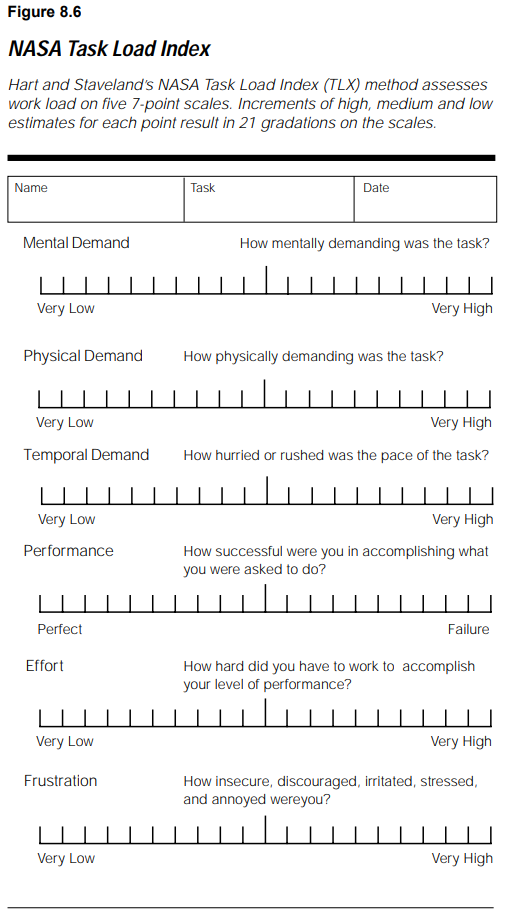
\includegraphics[width=0.78\linewidth]{obrazky-figures/nasaTLXform.png}
  \caption{NASA TLX (Task Load Index) - formulář pro subjektivní posouzení pracovní zátěže. Převzato z \cite{NasaTlx}.}
  \label{pic-nasaTlxForm}
\end{figure*}
\chapter{Paměťové médium}
Přiložené paměťové médium obsahuje zdrojové kódy rozhraní, propagační fotografie/videa a zdrojové kódy práce pro vytvoření PDF dokumentu.
\section{Demonstrační video}
Dle zadání vytvořené propagační video demonstrující klíčové vlastnosti řešení.
\section{Zdrojové kódy}
Médium obsahuje kompletní zdrojové kódy řešení včetně potřebných knihoven pro kompilaci a spuštění. Jsou zde přítomné i kódy pro vytvoření textové části práce.
\section{Shrnující plakát s přiloženým komentářem}
Plakát je ve formátu A1 a obsahuje souhrn informací o řešení.
  \fi
  
  % Kompilace po částech (viz výše, nutno odkomentovat)
  % Compilation piecewise (see above, it is necessary to uncomment it)
  %\subfile{projekt-30-prilohy-appendices}
  
\end{document}
